% --- V-JEPA 2 (Assran et al., arXiv:2506.09985) ---
\begin{frame}{V-JEPA 2: Scaling Video JEPA for Understanding and Planning}
  \begin{columns}[T,onlytextwidth]
    \column{0.42\textwidth}
    Same \textbf{visual mask denoising} / JEPA spirit as I-JEPA, but at \textbf{internet scale}.
    \vspace{0.2em}
      \begin{itemize}
          \item Order of \textbf{$\sim$1M hours} of video and \textbf{$\sim$1M images} for pre-training.
          \item Downstream use: video understanding, video QA, and planning.
      \end{itemize}
    \column{0.56\textwidth}
      \centering
      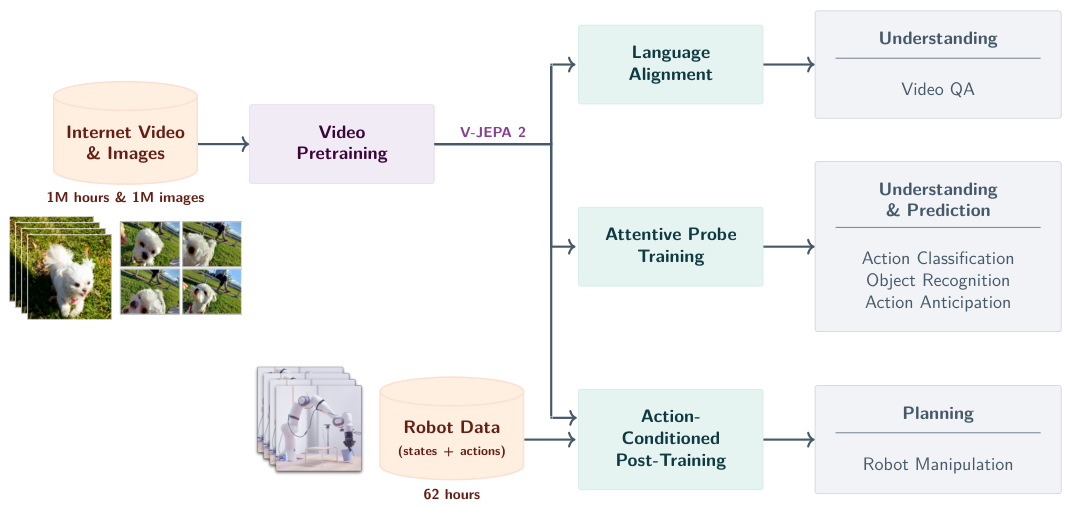
\includegraphics[width=0.9\linewidth,height=0.9\textheight,keepaspectratio]{images/jepa/vjepa2_paper_fig1_overview.png}
      {\scriptsize Assran et al.\ (2025): overview of pre-training, alignment, and robotics post-training.}
  \end{columns}
\end{frame}

\begin{frame}{V-JEPA 2: End-to-End System Overview}
  \begin{columns}[T,onlytextwidth]
    \column{0.35\textwidth}
    {\footnotesize
    \begin{itemize}\itemsep0.26em
      \item[\textcolor{red}{$\blacktriangleright$}] Stage \textbf{A:} SSL on web video/images $\rightarrow$ strong motion and appearance understanding.
      \item[\textcolor{red}{$\blacktriangleright$}] Stage \textbf{B:} \textbf{language alignment}: project video tokens into an LLM with small attentive stacks so the backbone supports VQA and reasoning.
      \item[\textcolor{red}{$\blacktriangleright$}] Stage \textbf{C:} optional \textbf{action-conditioned} head (V-JEPA 2-AC) on tens of hours of robot data for latent planning.
    \end{itemize}
    }
    \column{0.65\textwidth}
    \centering
    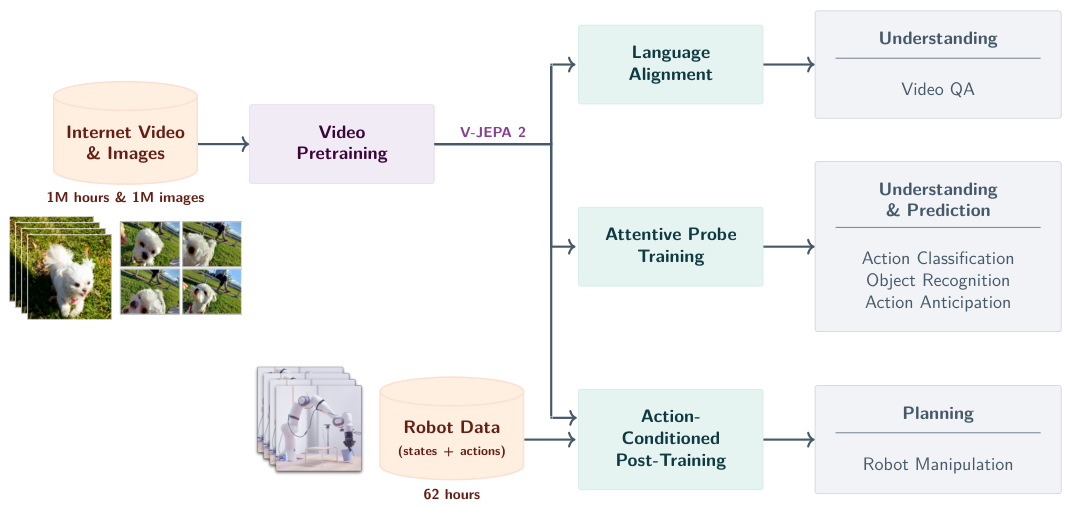
\includegraphics[width=0.9\linewidth,height=0.9\textheight,keepaspectratio]{images/jepa/vjepa2_paper_fig1_overview.png}
    {\scriptsize Overview of pre-training, alignment, and robotics post-training.}
  \end{columns}
  \vspace{-0.1em}

\end{frame}

% --- Vision-language grounding background (students skipped the Vision+Text lecture) ---
\begin{frame}{Connecting a Video Encoder to an LLM}
  \begin{itemize}\itemsep0.28em
    \item \textbf{Visual Question Answering (VQA):} answer natural-language questions about an image or video (``What is the person about to pick up?'').
    \item Standard recipe (LLaVA-style): keep the \textbf{vision encoder frozen} (or lightly tuned), train a small \textbf{projector} that maps visual tokens into the LLM's embedding space, then instruction-tune on paired visual--text data.
    \item V-JEPA 2 follows this pattern: \textbf{attentive pooling} compresses video tokens, a projector aligns them with an LLM ($\sim$8B parameters), and the coupled stack is trained on video--text data.
    \item Note that the JEPA encoder itself is \textbf{never trained on language}; grounding is added \emph{after} purely visual pre-training.
  \end{itemize}
\end{frame}

\begin{frame}{V-JEPA 2: Training Stage 1 (Pre-training)}
  \centering
  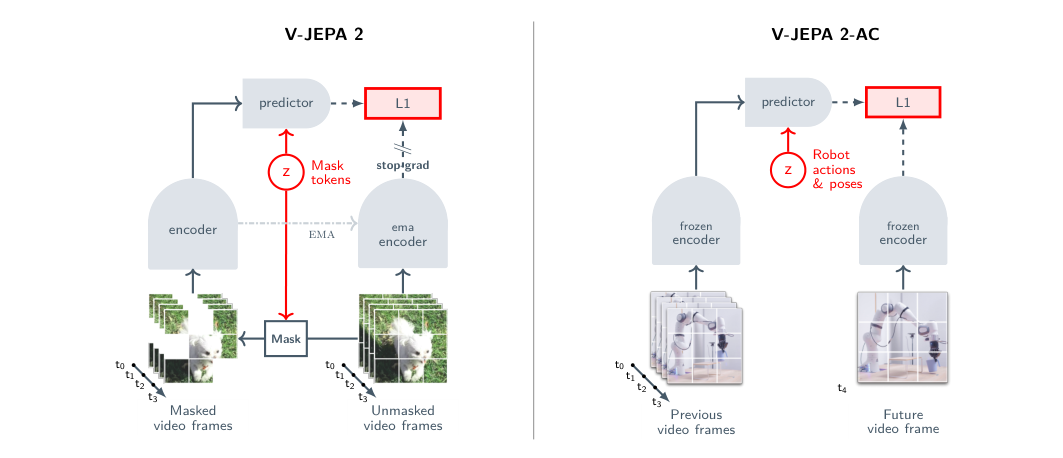
\includegraphics[width=0.9\linewidth,height=0.55\textheight,keepaspectratio]{images/jepa/vjepa2_paper_fig2_multistage.png}\\[0.25em]
  {\scriptsize Assran et al.\ (2025): multistage training.}
  {\footnotesize
  \begin{itemize}
    \item \textbf{V-JEPA 2:}
    \begin{itemize}   
      \item Video clips divided into tokens; a subset is masked.
      \item Encoder processes masked sequence to produce token embeddings.
      \item Mask tokens concatenated with encoder outputs.
      \item Predictor regresses to targets computed by an EMA encoder using $L_1$ loss.
    \end{itemize}
  \end{itemize}
  }
\end{frame}

\begin{frame}{V-JEPA 2: Training Stage 2 (Action-Conditioned)}
  \centering
  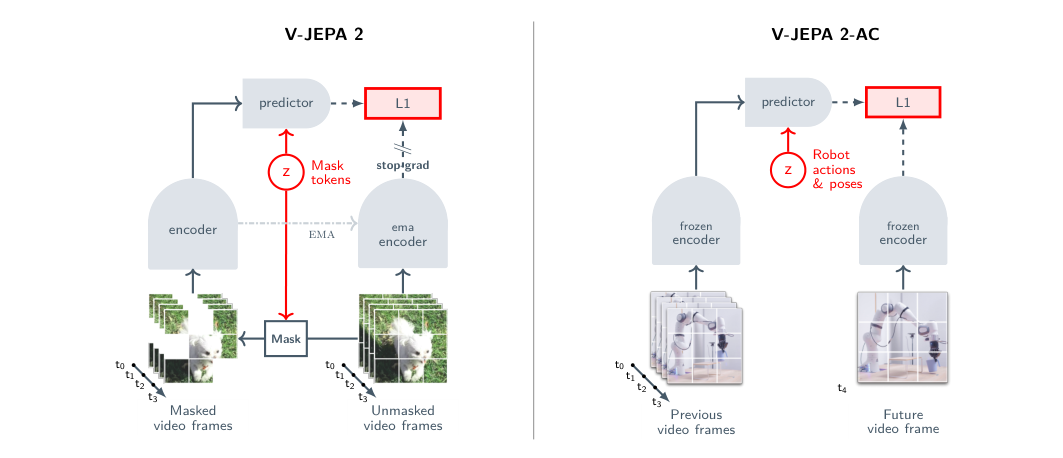
\includegraphics[width=0.9\linewidth,height=0.55\textheight,keepaspectratio]{images/jepa/vjepa2_paper_fig2_multistage.png}\\[0.25em]
  {\scriptsize Assran et al.\ (2025): multistage training.}
  {\footnotesize
  \begin{itemize}
    \item \textbf{V-JEPA 2-AC:}
    \begin{itemize}
      \item Freeze pretrained encoder and train action-conditioned predictor on top ($<$62 hours of unlabeled robot trajectories).
      \item Use autoregressive prediction to model future frame representations based on past frames, actions, and end-effector states.
    \end{itemize}
  \end{itemize}
  }
\end{frame}

% --- V-JEPA 2-AC: planning at inference (completes the robotics story) ---
\begin{frame}{V-JEPA 2-AC: Planning at Inference Time}
  Once the action-conditioned predictor is trained, it works as a \emph{simulator in representation space}, and \textbf{planning} requires no task-specific training.
  \vspace{0.3em}
  \begin{enumerate}\itemsep0.25em
    \item \textbf{Specify the goal as an image}; encode it to a goal representation $s_g$.
    \item \textbf{Sample candidate action sequences}; roll each out through the predictor to get predicted future representations.
    \item \textbf{Score} each rollout by the ($L_1$) distance between its predicted final state and $s_g$; refine the action distribution toward the best rollouts (\textbf{cross-entropy method, CEM}).
    \item \textbf{Execute only the first action}, observe, and \textbf{re-plan}: receding-horizon \textbf{model predictive control}, i.e.\ the multistep world-model loop shown earlier.
  \end{enumerate}
  \vspace{0.3em}
  \begin{itemize}\itemsep0.2em
    \item Result: \textbf{zero-shot} pick-and-place with Franka arms in labs \textbf{never seen in training}, with no rewards and no demonstrations in the target environment (as claimed in the paper).
  \end{itemize}
\end{frame}

\begin{frame}{V-JEPA 2: Performance}
  \centering
  \vspace{0.3em}
  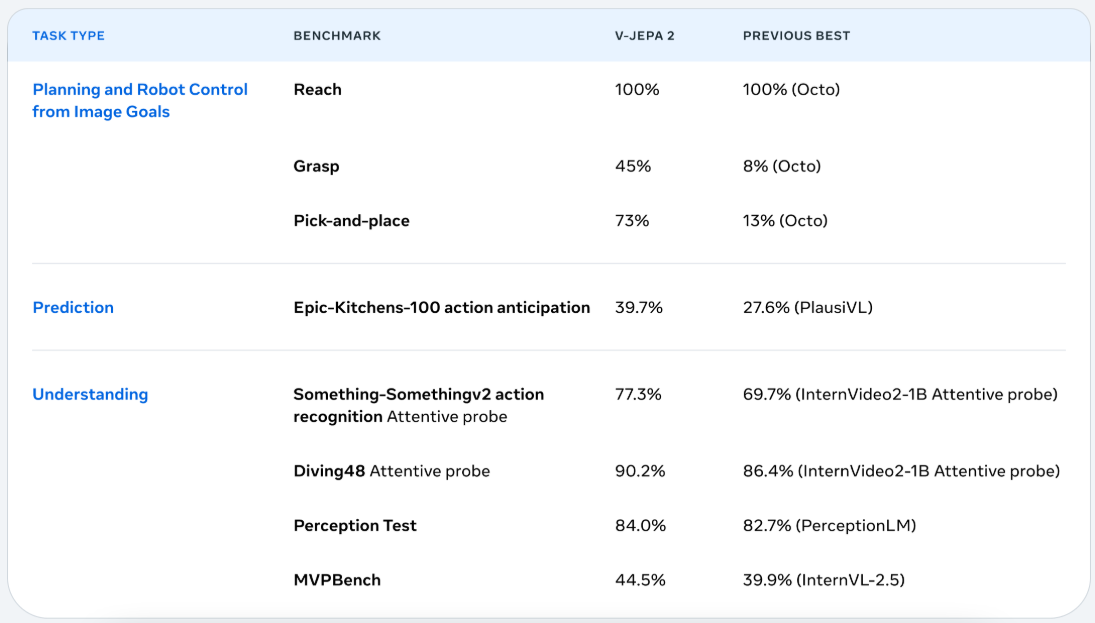
\includegraphics[width=0.9\linewidth,height=0.7\textheight,keepaspectratio]{images/jepa/vjepa2_paper_fig3_performance.png}
  \linebreak
  {\scriptsize Assran et al.\ (2025): performance; see also \href{https://ai.meta.com/research/vjepa/}{Meta AI V-JEPA blog post}.}
\end{frame}

\begin{frame}{V-JEPA 2: Headline Results}
  \begin{itemize}\itemsep0.28em
    \item[\textcolor{red}{$\blacktriangleright$}] \textbf{Fine-grained motion:} Something-Something v2 top-1 \textbf{77.3} (paper-reported).
    \item[\textcolor{red}{$\blacktriangleright$}] \textbf{Action anticipation:} Epic-Kitchens-100 recall@5 \textbf{39.7}, described as strong vs.\ prior task-specialized models.
    \item[\textcolor{red}{$\blacktriangleright$}] \textbf{Video QA (after LLM alignment):} e.g.\ PerceptionTest \textbf{84.0}, TempCompass \textbf{76.9} at an \textbf{8B-parameter} coupled stack (paper-reported).
    \item[\textcolor{red}{$\blacktriangleright$}] \textbf{Robotics:} V-JEPA 2-AC trained on \textbf{$<$62 hours} of Droid-style trajectories; \textbf{zero-shot} Franka pick--place demos in \textbf{unseen labs} without environment-specific teleoperation or task rewards (as claimed in the paper abstract).
  \end{itemize}
  {\scriptsize Treat numbers as \textbf{snapshot} results from Assran et al.; see \href{https://arxiv.org/pdf/2506.09985}{PDF} for protocols and ablations.}
\end{frame}
